\begin{frame}
\frametitle{Flux}
	\par
  	\textbf{Flux} è l’architettura che Facebook usa per creare applicazioni web client-side.\\
	\begin{flushleft}
		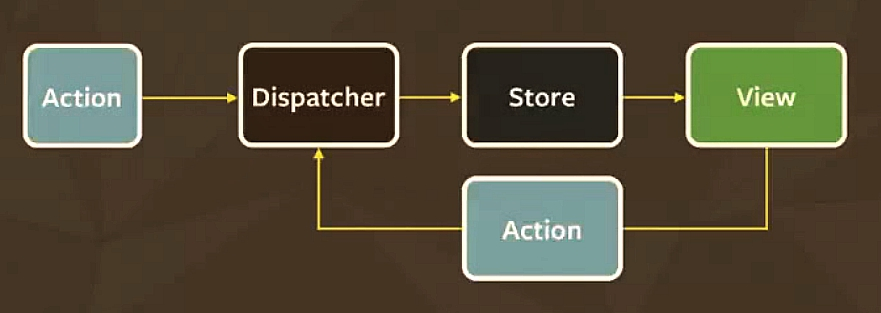
\includegraphics[scale=0.3]{n9.png}	
	\end{flushleft}	
	\textbf{Simile a MVC, ma...}\\
        Vuole prevenire cambiamenti “a cascata”, che portano a risultati difficilmente prevedibili se si usa il pattern MVC su larga scala.
\end{frame}


